\documentclass[
    bibsize = normalsize,
    bibpackage = none,
    paragraphshape = display,
    paragraphafter = none,
]{goose-article}

\usepackage[backend=bibtex, style=numeric, sorting=ydnt]{biblatex}

\usepackage{eurosym}
\usepackage{setspace}
\usepackage{enumitem}
\setlist[enumerate]{itemsep=0mm}

\title{Curriculum Vitae}
\author{Tom de Geus}
\date{}

\newcommand{\MYhref}[3][Blue]{\href{#2}{\color{#1}{#3}}}%

\newcounter{magicrownumbers}
\newcommand\rownumber{\stepcounter{magicrownumbers}\arabic{magicrownumbers}}

\usepackage{array}
\usepackage{etoolbox}

% \begin{noindent}
\newcommand{\PreserveBackslash}[1]{\let\temp=\\#1\let\\=\temp}
\newcolumntype{C}[1]{>{\PreserveBackslash\centering}p{#1}}
\newcolumntype{R}[1]{>{\PreserveBackslash\raggedleft}p{#1}}
\newcolumntype{L}[1]{>{\PreserveBackslash\raggedright}p{#1}}
% \end{noindent}

\renewcommand{\arraystretch}{1.3}

% --------------------------------------------
% https://tex.stackexchange.com/a/22770/132350

% Count total number of entries in each refsection
\AtDataInput{%
    \csnumgdef{entrycount:\therefsection}{%
        \csuse{entrycount:\therefsection}+1
    }
}

% Print the labelnumber as the total number of entries in the
% current refsection, minus the actual labelnumber, plus one
\DeclareFieldFormat{labelnumber}{\mkbibdesc{#1}}
\newrobustcmd*{\mkbibdesc}[1]{%
    \number\numexpr\csuse{entrycount:\therefsection}+1-#1\relax
}

% --------------------------------------------

\addbibresource[label=publications]{library_publications.bib}
\addbibresource[label=invited]{library_invited.bib}
\addbibresource[label=conferences]{library_conferences.bib}
\addbibresource[label=posters]{library_posters.bib}
\addbibresource[label=seminars]{library_seminars.bib}
\addbibresource[label=students]{library_students.bib}

\begin{document}

\maketitle

\begin{center}
    ``It's not the answers you give, but the questions you ask'' -- Voltaire
\end{center}

\section*{Personal information}

\vspace*{-1eM}
\begin{minipage}[c]{.7\textwidth}
    Dr.ir.\ Tom de Geus\\
    Chemin du Parc-de-Valency 11, 1004 Lausanne, Switzerland\\
    \MYhref{mailto:tom@geus.me}{tom@geus.me}, +41 77 993 72 35, % Please find me on:
    \MYhref{http://www.geus.me}{www.geus.me} \\
    Dutch (mother tongue), \\
    English (fluent), French (fluent), \\
    German (passive B2/C1, active A2/B1)
\end{minipage}
\begin{minipage}[c]{.3\textwidth}
    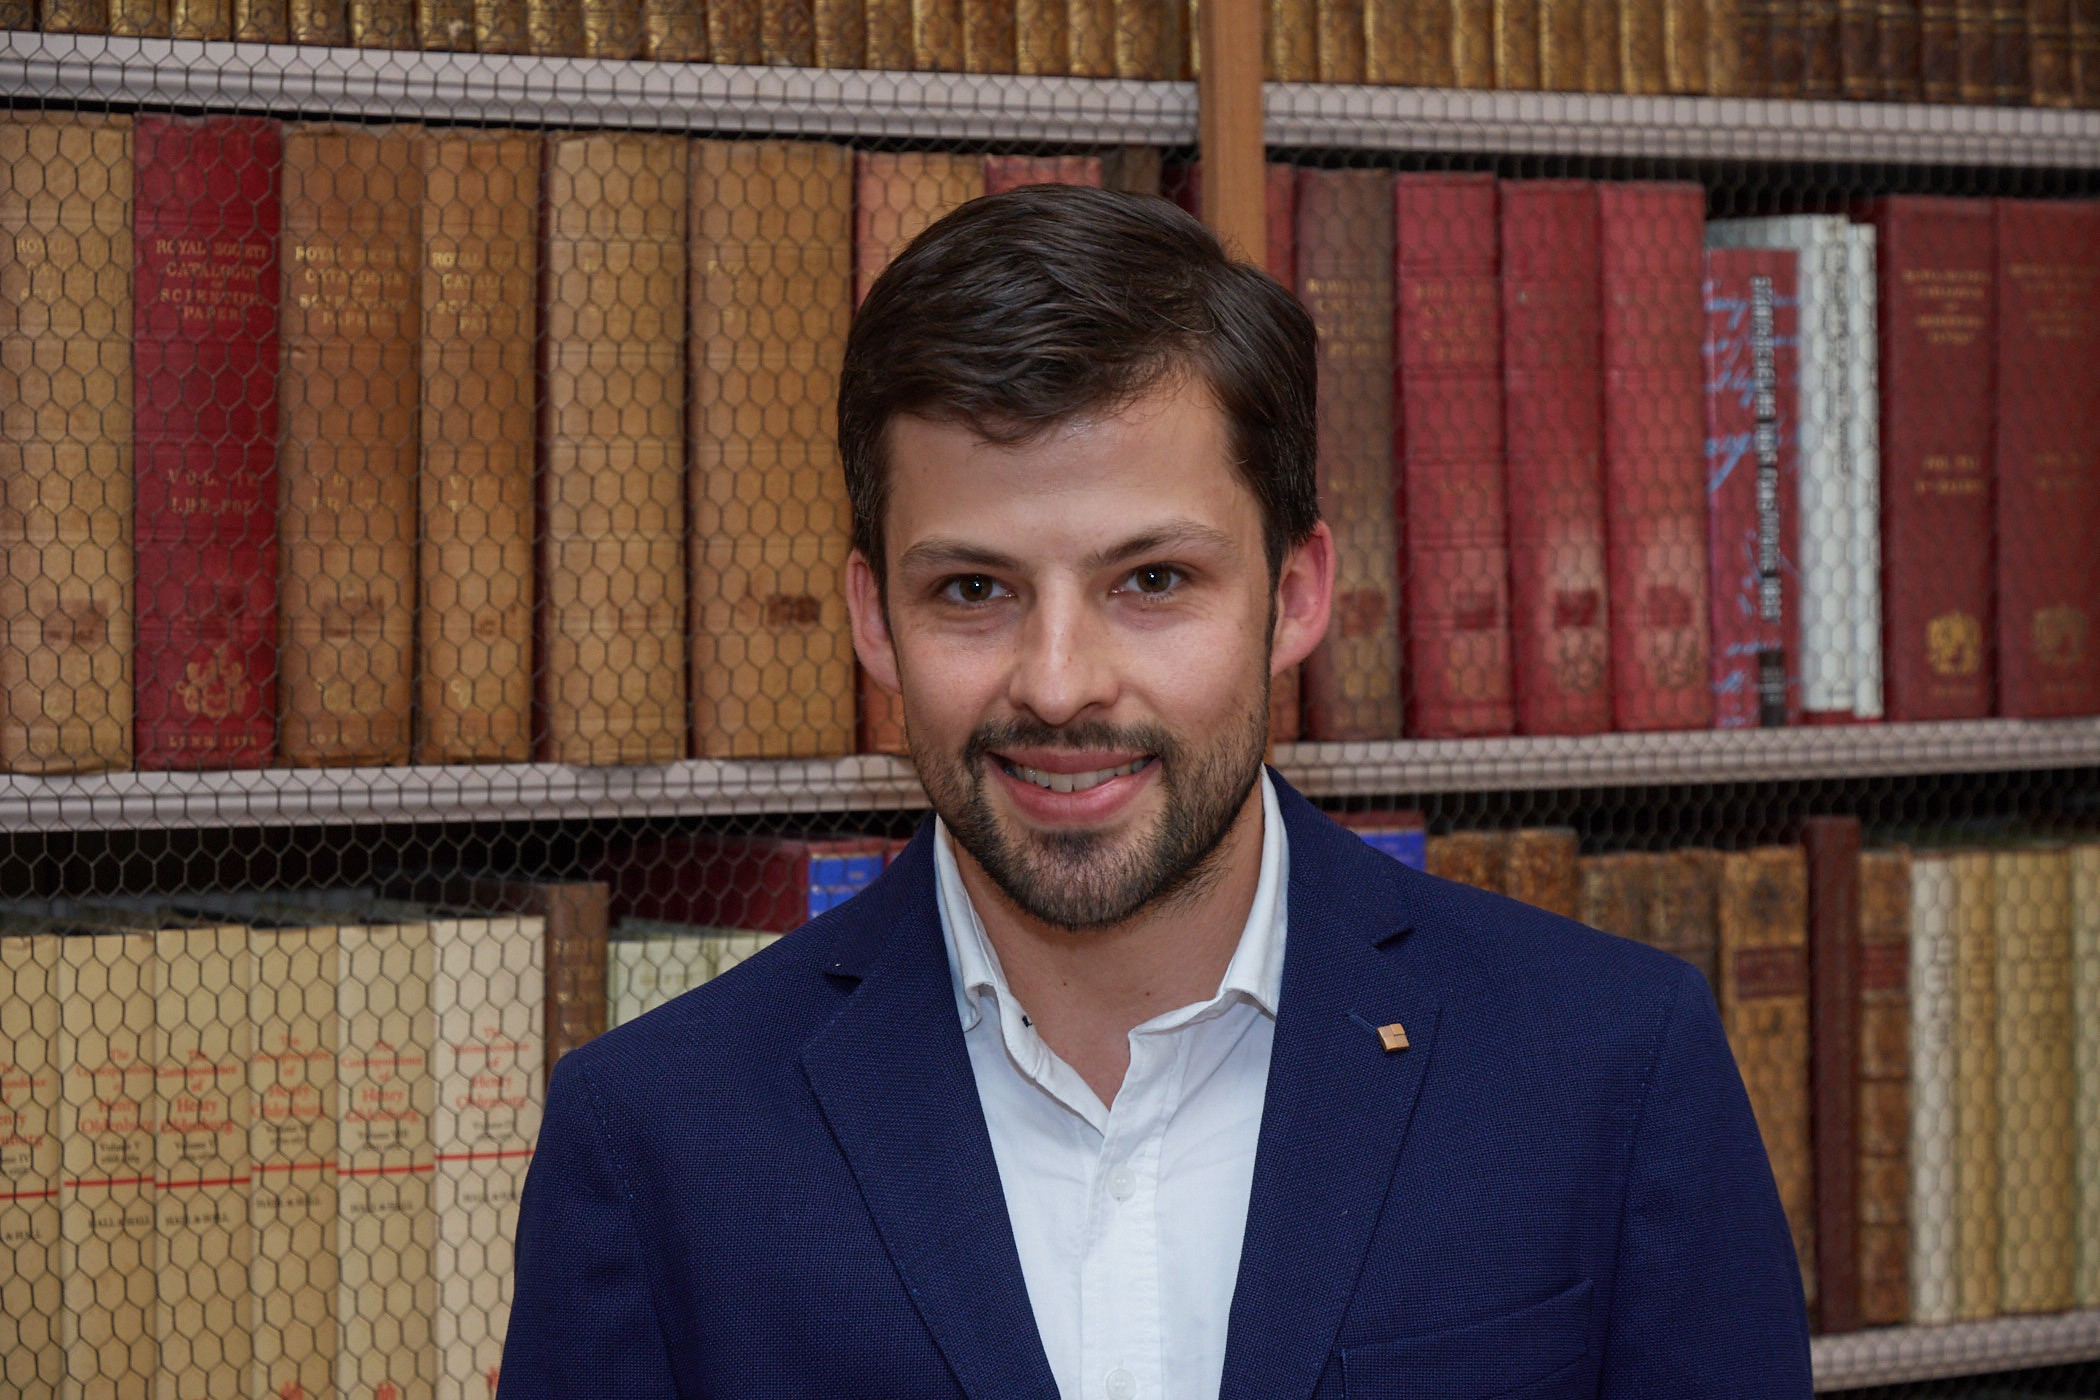
\includegraphics[width=\textwidth]{figures/tom.jpg}
\end{minipage}
\vspace*{-1.5eM}

\section*{Education}

\noindent
\preto\tabular{\setcounter{magicrownumbers}{0}}
\begin{tabular}{L{4mm}L{129mm}R{27mm}}
    % ---------
    \rownumber.
     &
    PhD Mechanical Engineering (\emph{cum laude}). Defended: 03.05.2016.\newline
    Promotor: Prof.dr.ir.~Marc~Geers, co-promotor: Dr.ir.~Ron~Peerlings.\newline
    Eindhoven University of Technology (TU/e), The Netherlands.
     &
    04.2012 -- 04.2016
    % ---------
    \\
    % ---------
    \rownumber.
     &
    Graduate School Engineering Mechanics.\newline
    Supported by 3TU (Joint Universities of Technology in The Netherlands).
     &
    04.2012 -- 10.2015
    % ---------
    \\
    % ---------
    \rownumber.
     &
    Master Mechanical Engineering (\emph{with great appreciation}).\newline
    Thesis directors: Prof.dr.ir.~Marc~Geers, dr.ir.~Ron~Peerlings.\newline
    Eindhoven University of Technology, The Netherlands.
     &
    09.2009 -- 08.2012
    % ---------
    \\
    % ---------
    \rownumber.
     &
    Internship (\emph{excellent evaluation}).\newline
    Director: Prof.dr.~Katia Bertoldi.\newline
    Harvard University, School of Engineering and Applied Sciences, Cambridge, USA.
     &
    09.2010 -- 11.2010
    % ---------
    \\
    % ---------
    \rownumber.
     &
    Bachelor Mechanical Engineering (\emph{with great appreciation}).\newline
    Minor: entrepreneurship.\newline
    Eindhoven University of Technology, The Netherlands.
     &
    09.2004 -- 12.2009
    % ---------
    \\
    % ---------
    \rownumber.
     &
    Pre-university secondary education.\newline
    Specialisation: science and technology.\newline
    Lorentz Casimir Lyceum, Eindhoven, The Netherlands.
     &
    09.1997 -- 06.2004
    % ---------
\end{tabular}

\section*{Employment history (academic positions only)}

\noindent
\preto\tabular{\setcounter{magicrownumbers}{0}}
\begin{tabular}{L{4mm}L{129mm}R{27mm}}
    % ---------
    \rownumber.
     &
    Ambizione fellow (see fellowships).\newline
    Institute of Physics, \'{E}cole Polytechnique F\'{e}d\'{e}rale de Lausanne (EPFL), CH.
     &
    10.2019 -- current
    % ---------
    \\
    % ---------
    \rownumber.
     &
    Rubicon post-doc fellow (see fellowships).\newline
    Director: Prof.dr.~Matthieu Wyart.\newline
    Institute of Physics, \'{E}cole Polytechnique F\'{e}d\'{e}rale de Lausanne (EPFL), CH.
     &
    09.2016 -- 10.2019
    % ---------
    \\
    % ---------
    \rownumber.
     &
    Post-doc (valorisation project for M2i and TATA Steel Europe).\newline
    Director: Prof.dr.ir.~Marc~Geers.\newline
    Department of Mechanical Engineering, Eindhoven University of Technology, NL.
     &
    04.2016 -- 07.2016
    % ---------
    \\
    % ---------
    \rownumber.
     &
    PhD researcher.\newline
    Directors: Prof.dr.ir.~Marc~Geers, dr.ir.~Ron~Peerlings.\newline
    Department of Mechanical Engineering, Eindhoven University of Technology, NL.\newline
    Materials Innovation Institute (M2i), Delft, NL.
     &
    04.2012 -- 04.2016
    % ---------
\end{tabular}

\section*{Prizes, awards, fellowships}

\paragraph{Prizes}

\noindent
\preto\tabular{\setcounter{magicrownumbers}{0}}
\begin{tabular}{L{4mm}L{129mm}R{27mm}}
    % ---------
    \rownumber.
     &
    Martinus van Marum award for best PhD thesis in the engineering sciences \newline
    in a period of five years, Koninklijke Hollandsche Maatschappij der Wetenschappen \newline
    (Royal Holland Society of Sciences and Humanities). \newline
    Prize: acceptance colloquium, a medal, and 12500 \euro.
     &
    06.2017
    % ---------
    \\
    % ---------
    \rownumber.
     &
    Best PhD thesis in Mechanical Engineering of the calendar year 2016, \newline
    Eindhoven University of Technology (TU/e). Prize: 250 \euro.
     &
    05.2017
    % ---------
\end{tabular}

\paragraph{Awards}

\noindent
\preto\tabular{\setcounter{magicrownumbers}{0}}
\begin{tabular}{L{4mm}L{129mm}R{27mm}}
    % ---------
    \rownumber.
     &
    Winner of the 7th ECCOMAS PhD Olympiad. \newline
    Award: 500 \euro.
     &
    09.2017
    % ---------
    \\
    % ---------
    \rownumber.
     &
    Poster award for best innovative research value, \newline
    M2i annual research conference. Award: 250 \euro.
     &
    12.2016
    % ---------
    \\
    % ---------
    \rownumber.
     &
    Poster award, \newline
    M2i annual research conference. Award: 250 \euro.
     &
    12.2013
    % ---------
    \\
    % ---------
    \rownumber.
     &
    Entrepreneurship award for best business case, \newline
    Eindhoven University of Technology. Award: 1000 \euro.
     &
    02.2008
\end{tabular}

\paragraph{Fellowships}

\noindent
\preto\tabular{\setcounter{magicrownumbers}{0}}
\begin{tabular}{L{4mm}L{129mm}R{27mm}}
    % ---------
    \rownumber.
     &
    Ambizione fellowship, Grant No.\ PZ00P2{\_}185843 \newline
    Swiss National Science Foundation (FNSF). Grant: 567 kCHF.
     &
    09.2019
    \\
    % ---------
    \rownumber.
     &
    Rubicon fellowship, Grant No.\ 680-50-1520 \newline
    The Netherlands Organisation for Scientific Research (NWO). Grant: 160 k\euro.
     &
    09.2016
    % ---------
\end{tabular}

\begin{refsection}[publications]
    \nocite{*}
    \printbibliography[locallabelwidth, title={Publications (chronological)}]
\end{refsection}

\begin{refsection}[invited]
    \nocite{*}
    \settoggle{bbx:url}{false}
    \printbibliography[locallabelwidth, title={Conferences (invited oral)}]
\end{refsection}

\begin{refsection}[conferences]
    \nocite{*}
    \settoggle{bbx:url}{false}
    \printbibliography[locallabelwidth, title={Conferences (oral)}]
\end{refsection}

\begin{refsection}[posters]
    \nocite{*}
    \settoggle{bbx:url}{false}
    \printbibliography[locallabelwidth, title={Conferences (posters)}]
\end{refsection}

\begin{refsection}[seminars]
    \nocite{*}
    \settoggle{bbx:url}{false}
    \printbibliography[locallabelwidth, title={Colloquia (invited)}]
\end{refsection}

\begin{refsection}[students]
    \nocite{*}
    \settoggle{bbx:url}{false}
    \printbibliography[locallabelwidth, title={(Co-)Supervised junior researchers: PhD, master, bachelor (chronological)}]
\end{refsection}

\section*{Teaching activities (chronological)}

\begin{enumerate}
    \itemsep0em
    \item Teaching assistant ``Statistical Physics 2'' (bachelor, EPFL, 02.2020 -- 07.2020)
    \item Teaching assistant ``Continuum Mechanics'' (bachelor, EPFL, 09.2016 -- 02.2017)
    \item Lecturer ``Programming project'' (bachelor, TU/e, 09.2011 -- 09.2015)
    \item Teaching assistant ``Finite Element Method'' (bachelor, TU/e, 09.2010 -- 09.2011)
    \item Co-developer of a tensor toolbox in Matlab for education purposes (TU/e, 09.2009 -- 09.2010)
    \item Supervisor ``Design Based Learning'' (bachelor, TU/e, 09.2008 -- 09.2009)
\end{enumerate}

\section*{Scientific reviewing activities (journals, alphabetical)}

\begin{itemize}
    \item Computational Materials Science
    \item Computer Methods in Applied Mechanics and Engineering
    \item Engineering Fracture Mechanics
    \item International Journal of Numerical Methods in Engineering
    \item International of Journal of Fracture
    \item Journal of the Mechanics and Physics of Solids
    \item Mechanics of Materials
    \item Modelling and Simulation in Materials Science and Engineering
    \item Nature Communications
    \item Numerical Algorithms
    \item Physical Review E
    \item Physical Review Letters
    \item Strain
\end{itemize}

\section*{Organisation of conferences (chronological)}

\begin{enumerate}
    \item Co-organiser of colloquium of Dr.\ Elsa Bayart at EPFL (10.2023).
    \item Co-organiser of colloquium of Prof.dr.\ Jan Zeman at EPFL (09.2017).
\end{enumerate}

\section*{Institutional responsibilities (chronological)}

\begin{enumerate}
    \itemsep0em
    \item Data champion (EPFL, 09.2021 -- current).
    \item Cluster administrator for the Physics of Complex Systems Laboratory (EPFL, 03.2017 -- current).
    \item Founder of computing cluster support and professionalisation panel (TU/e, 09.2013 -- 07.2016).
\end{enumerate}

\section*{Outreach activities (chronological)}

\begin{enumerate}
    \itemsep0em
    \item \MYhref{https://pages.rts.ch/la-1ere/programmes/forum/11247813-forum-du-22-04-2020.html}{Radio interview Swiss National Television (RTS)} (22.04.2020).
    \item Interview by freelance journalist Janny Terlouw (text available on \MYhref{http://www.geus.me/career/2017/06/13/khmw-martinus-van-marum-prijs.html}{www.geus.me}) (05.2017).
    \item Radio interview Rradio (05.2016).
\end{enumerate}

\section*{Programming}

\begin{itemize}
    \itemsep0em
    \item Expert: C++, Python, LaTeX.
    \item Extensive experience: C, Fortran, OpenMP, Matlab, Bash, Qt.
    \item Maintainer open-source projects: \MYhref{https://github.com/xtensor-stack/xtensor}{xtensor}, \MYhref{https://github.com/bluebrain/HighFive}{HighFive}, \MYhref{https://github.com/sciunto-org/python-bibtexparser}{python-bibtexparser}.
    \item Developed libraries (selection): \MYhref{https://github.com/tdegeus/GooseFEM}{GooseFEM}, \MYhref{https://github.com/tdegeus/GooseEYE}{GooseEYE}, \MYhref{https://github.com/tdegeus/texplain}{texplain}, \MYhref{https://github.com/tdegeus}{\dots}.
\end{itemize}

\section*{Volunteering}

\begin{itemize}
    \itemsep0em
    \item Assistant group leader tour skiing, Alpine Club Switzerland, Lausanne (CH, 2024 -- current).
    \\
    Responsibilities: tour planning, assurance of safety.
    \item Member Commission leisure rowing, Lausanne Sport Aviron, Lausanne (CH, 2019 -- current).
    \\
    Responsibilities: group leader outing supervisors leisure rowing, planning and execution travels.
    \item Outing supervisor leisure rowing, Lausanne Sport Aviron, Lausanne (CH, 2019 -- current).
    \\
    Responsibilities: team formation, coaching, assurance of safety.
    \item President Hora Est, PhD association for (bio-)mechanical engineering (NL, 2014 -- 2015).
    \\
    Responsibilities: design and execution social events and career events.
    \item Buddy of autistic first year student (NL, 2008 -- 2009).
    \\
    Responsibilities: enhance well-being and study-effectiveness of autistic student.
    \item Field hockey equipment commissioner, Eindhoven area (NL, 2003 -- 2007).
    \\
    Responsibilities: purchase and maintenance of goalkeeper equipment (budget: 8000 euro per year).
    \item Trainer field hockey, Eindhoven area (NL, 2005 -- 2010).
    \\
    Responsibilities: design and execution specialised goalkeeper training.
\end{itemize}

\section*{Student jobs}

\begin{itemize}
    \itemsep0em
    \item Tutor of high school students in physics and math, Eindhoven area (NL, 09.2004 -- 09.2008).
    \item Sales employee and driver for an industrial rental company, Boels rental (NL, 09.2003 -- 09.2007).
    \item Shift supervisor hospitality, Maison van den Boer at soccer stadium of PSV (NL, 09.2001 -- 09.2004).
\end{itemize}

\section*{Other activities}

\begin{itemize}
    \itemsep0em
    \item Tour du L\'{e}man (longest row race in the world on closed water) (CH, 09.2022, 09.2023).
    \item Swiss Champion Rowing, Master Men 4x (CH, 07.2023).
    \item Bronze Medal Swiss Championships Rowing, Master Men 2x (CH, 07.2021).
    \item Goalkeeper first squad field hockey, Eindhoven area (NL, 2003 -- 2015).
\end{itemize}

\end{document}
